\section{Instrumentation}

There are two main challenges on tracing the progress of a process with binary instrumentation
in production systems. One challenge is performance. Even a lightweight static binary
instrumentation would increases execution time by tens of percentages. The other one is
progress accuracy. The ideal progress tracing rate is uniform along the whole execution, which
means that it can estimate accurately how much the task has been done and how long it
lasts. Take downloading a file for example. If the downloading progress bar shows a
50\% completion after 1 minute, it is clear that half of the task has been done and it may
last another 1 minute with a stable network connection. But for a compute-intensive
process, we only know that the process has met which tracepoint we instrumented. We can
not know the actions of the process that have no instrumented tracepoints, and the same
to the subsequent actions of the process. In a word, it is hard to estimate the progress of a compute-intensive
process that is not related to data I/O.

We primarily concern the performance of tracing in $NO^2$'s instrumentation, and 
overcome the accuracy issue with our outlier clustering solution which does not rely on
accurate estimation of progress. This will be discussed in the next section.

After many case studies, we have got two simple observations on binary code runtime
behaviors. Functions in a binary can be placed on different levels of an abstract syntax
tree (AST). Functions on the same level of AST are often called at similar frequency, and
the minority of the functions on the low level of AST consumes the majority of execution time
following a Pareto principle (80/20 principle). Table \ref{table:inst-stats} shows
the statistics of function hits of the instrumented ImageMagick dynamic link library.
There are 1060 functions in the library and only 33 functions are called by more than 10,000
times in five executions.

\begin{table}[h]
\caption{Statistics of function hits of ImageMagick}
\label{table:inst-stats}
\begin{center}
\begin{tabular}{r|r|l}
\hline
Hits & Functions & Example \\
\hline
above $10^7$ & 6 & CopyMagickMemory \\
$10^6$ - $10^7$ & 16 & GetCacheNexus \\
$10^5$ - $10^6$ & 2 & LocaleCompare \\
$10^4$ - $10^5$ & 9 & GetNexus \\
$10^3$ - $10^4$ & 10 & AddValueToSplayTree \\
$10^2$ - $10^3$ & 17 & FormatMagickStringList \\
$10^1$ - $10^2$ & 78 & NewSplayTree \\
$0$    - $10^1$ & 922 & GaussianBlurImage \\
\hline
\end{tabular}
\end{center}
Note: Only one function of each order of magnitude is shown in the table for example.
\end{table}

As we know, the entry/exit points of functions and basic blocks are commonly used
instrument points. For the purpose of progress tracing, an idealistic idea is to instrument 
each entry and exit point with all functions and basic blocks. Apparently, the overhead is
proportional to the hit rates. So with a few more coarse-grained instrumentations, we
can skip the minority of functions and reduce the majority of overheads. With the wish of minimum
overheads, we proposed a hit-statistics based function instrument
approach. This goal has been achieved as the evaluation section shows.

The instrument point selector is designed to record each function call and maintain the
function hits statistics which are saved in a key-value pattern: function name and number of
calls. After several runs, different AST levels of functions can be distinguished
according to the function hits. The instrumenter first loads the statistics data and
calculates the mean of hit numbers of all functions. Then it inserts a code snippet at
entries of each function, but skips those with a larger number of hits than the mean.
If it works well, the mean of all function hits will be set as the customized
threshold. With the automatic selection, the instrumenter can instrument the
binary codes in an appropriate granularity. The instrumented binary is written back as
a seperate file and sent to the ProActive scheduler to execute.

\section{Outlier Clustering}

For speculative executions, the first task of $NO^2$ is finding out the outliers.
With the traces returned by the instrumented processes, $NO^2$ uses an approach based on
Kmeans Clustering algorithm, which is commonly used in statistics analysis and data
mining, to hunt the outliers. With outliers exposed, $NO^2$ performs speculative
executions which needs to interact with the job scheduler.

There are several assumptions for the outliers clustering.

\begin{itemize}
\item Outliers is the minority of the massive parallel processes.
\item The tasks are split with a small amount of imbalance.
\item The server nodes of cluster becomes abnormal indeterminately and may return to
normal after a while.
\end{itemize}

We novelly select two properties of each process's traces to make outliers exposed, the
number of tracepoints met $N$ and the increment of tracepoints in one interval
$I$. Figure \ref{figure:executionsexample} shows a possible example of two processes of
the same binary code with same input at runtime. Ideally they should draw the same line,
but process B is actually slower than process A. It is similar to the accuracy test of
instrumentation in the evaluation section.

\begin{figure}
\centering
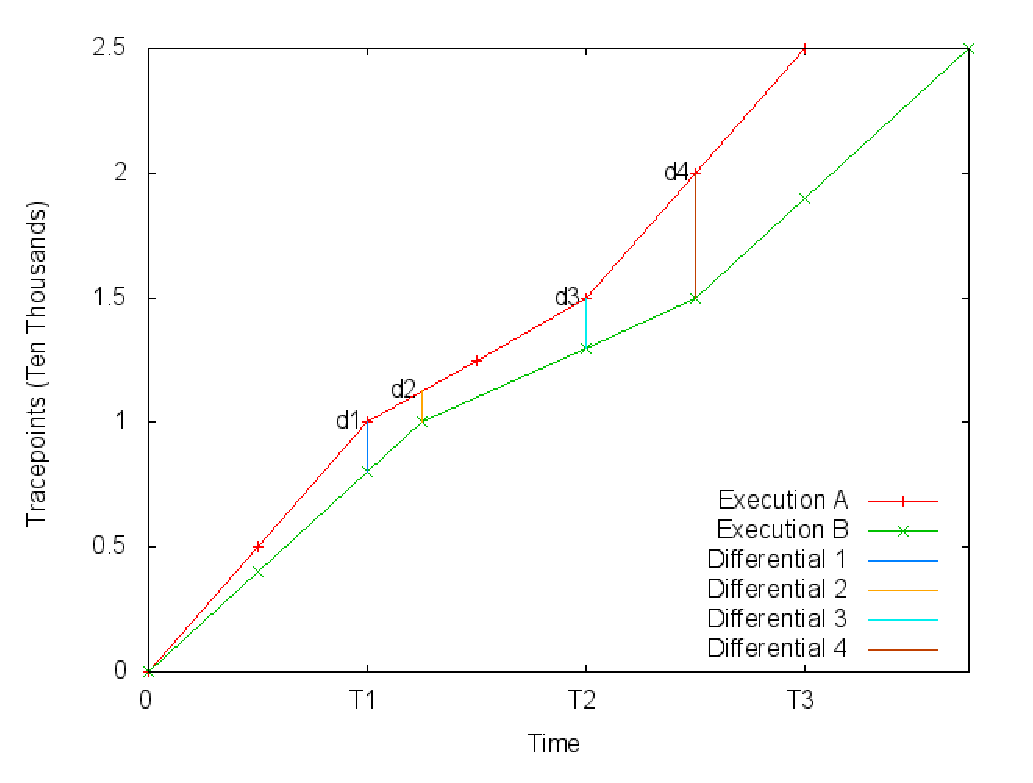
\includegraphics[width=0.9\columnwidth]{figures/executions_example.eps}
\caption{Tracepoints of two example executions}
\label{figure:executionsexample}
\end{figure}

A idealistic idea for exposing outliers is generating two clusterings using a one-degree Kmeans
Clustering algorithm with all processes' number of tracepoints. And if the normalized
variation of the two clusterings' means is larger than a threshold $T$, the clustering of
processes with a mean value of $N$ less than the other one will be judged as outliers.

But the number of tracepoints is increased unevenly. We have mentioned this dilemma at the
instrumentation section. Four differences of two processes' number of tracepoints has been
marked as $d_1, d_2, d_3, d_4$ at four different time points. Although process B is always
0.8X slower than process A, the difference of process A and process B is not increased
along the whole time line. An obvious case is $d_1 > d_2$, this may lead to the naive
kmeans clustering approach missing process B when clustering outliers. Another type of
mistake is some conditions just as $d_3 < d_4$. Process B may be just a little slower than
process A, but it is judged as an outlier in the naive kmeans clustering approach. So there no
fixed threshold $T$ which is appropriate for judging the outliers with the naive kmeans
clustering approach.

To eliminate the mistake caused by false positives and false negatives, an improved approach
has been proposed in $NO^2$. We proposed a new dynamic threshold $T_d$, which is
determined by the threshold $T$, the mean of all processes' tracepoints increment $I_m$
and the $i$th process's tracepoints increment $I_i$.

$$T_d = T \cdot (I_m / I_i)$$

As one of the assumptions is that outliers is the minority, the mean of the increment of
tracepoints of all processes $I_m$ is nearly the same to the majority. When the variance
of the means of clusterings decreased exceptionally like the case $d_1 > d_2$, the dynamic
threshold $T_d$ decreased correspondingly. When the variance of the means of clusterings
increased exceptionally like the case $d_3 < d_4$, the corresponding increase of $T_d$
comes along. So dynamic threshold $T_d$ can generally be adaptive to the uneven increase of the number
of tracepoints. With this improved approach for outliers clustering, $NO^2$
can find out most outliers whereas introduces few false positives. 
